\subsection{Local Similarity Search on Geolocated Time Series}
\label{sec:problem}

Next, we briefly present some background on geolocated time series and the \btsr index, and then formally define the problem. 

% Next, we briefly present the preliminaries that we used, followed by our formal problem definition.

\subsubsection{Preliminaries}
\label{subsec:preliminaries}

\noindent \textbf{\emph{Geolocated Time Series}}. A {\em time series} is a time-ordered sequence of values $T = \{T^1, T^2 \ldots, T^{n}\}$, where $T^{i}$ is the value at the $i$-th timestamp and $n$ is the length of the series. A geolocated time series is additionally characterized by a \emph{location}, denoted by $T.loc$. The {\em spatial distance} $d$ between two geolocated time series is the Euclidean distance of their respective locations.
% Assuming a 2-dimensional space, we further use the notation $T.loc_x$, $T.loc_y$ to refer to the $(x,y)$ coordinates of $T$. 
% :

% \begin{equation} \label{eq:dist_sp2}
% d(T, T') = \sqrt{(T.loc_x - T'.loc_x)^2 + (T.loc_y - T'.loc_y)^2}
% \end{equation}

% In this paper, we consider sets of {\em co-evolving} geolocated time series, so all time series are {\em time-aligned} (i.e., they contain observation values at the same timestamps all along their duration.) and each series has a value at each of the $k$ timestamps.


% \noindent \textbf{\emph{Minimum Bounding Time Series.}} \checknote{
\noindent \textbf{\emph{The \btsr Index}}. In \cite{chatzig17btsr}, we have introduced the \btsr index, which is based on the notion of {\em Minimum Bounding Time Series} (MBTS). In a similar manner that an MBR encloses a set of geometries, an MBTS encloses {\em a set of time series} $\mathcal{T}$ using a pair of bounds that fully contain all of them. Figure~\ref{fig:example_bundle} depicts an example of two MBTSs for two disjoint sets of time series. Formally, given a set of time series $\mathcal{T}$, its MBTS consists of an \emph{upper bounding time series} $B^{\sqcap}$ and a \emph{lower bounding time series} $B^{\sqcup}$, constructed by respectively selecting the maximum and minimum of values at each timestamp $i \in \{ 1, \dots, n\}$ among all time series in set $\mathcal{T}$ as follows:

\begin{align}\label{eq:bounds1}
 \begin{split}
  & B^{\sqcap} = \{ \max_{T \in \mathcal{T}} T^1, \ldots, \max_{T \in \mathcal{T}} T^n \} \\
  & B^{\sqcup} = \{ \min_{T \in \mathcal{T}} T^1, \ldots, \min_{T \in \mathcal{T}} T^n \}
 \end{split}
\end{align}

\begin{figure}[tb]
    \centering
    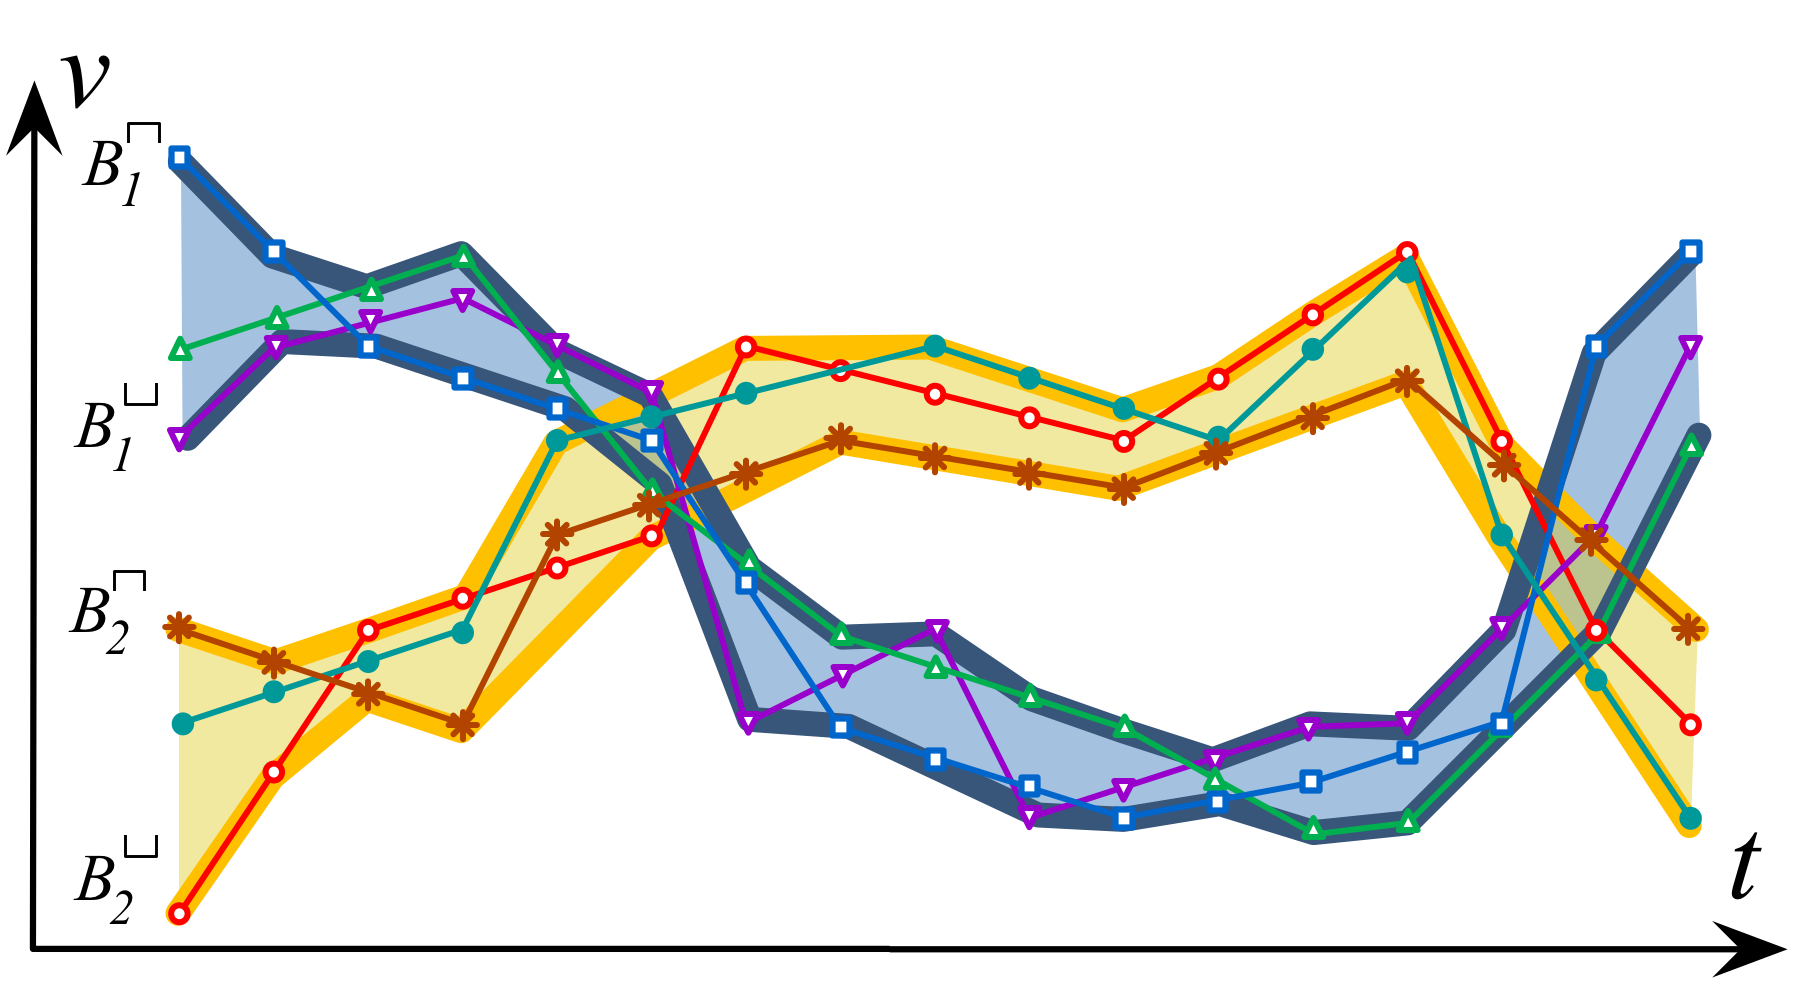
\includegraphics[width=75mm]{Figures/mbts.png}
    \caption{MBTS constructed for two sets of time series.}
    \label{fig:example_bundle}
\end{figure}

% Note that both bounding time series have the same length $n$ as those enclosed within this MBTS.
% }

% \noindent \textbf{\emph{The \btsr Index.}} \checknote{
A \btsr index is initialized as an R-tree \cite{Guttman1984} built on the spatial attributes of the given geolocated time series dataset, as depicted in the example of Figure~\ref{fig:example}. Besides MBRs, each node is enhanced to also store MBTSs, shown as colored strips per node in Figure~\ref{subfig:btsrtree}. This enables efficient pruning of the search space when evaluating hybrid queries combining time series similarity with spatial proximity.
% As in R-trees, each node of the \btsr has at least $m$ and at most $M$ entries and stores the MBRs of its children. Additionally, f
For each child, a node stores a pre-specified number of MBTSs. Each MBTS is calculated according to Eq.~\ref{eq:bounds1}. Construction and maintenance of the \btsr follow the procedures of the R-tree for data insertion, deletion and node splitting. Objects (i.e., geolocated time series) are inserted into leaf nodes and any resulting changes are propagated upwards. Once the nodes have been populated, the MBTS of each node are calculated bottom-up, relying on $k$-\textit{means clustering} according to their Euclidean distance in the time series domain. The example in Figure \ref{fig:example_bundle} depicts the $k=2$ MBTSs (as two bands with a thick outline) obtained for a set of time series (shown as thin polylines). In a \btsr, each parent node receives all the MBTSs of its children and computes its own $k$ MBTSs. The process continues upwards, until reaching the root.

\begin{figure}[!t]
 \centering
\begin{minipage}[!t]{0.5\linewidth}
 \subfloat[Sample dataset with MBRs over locations]{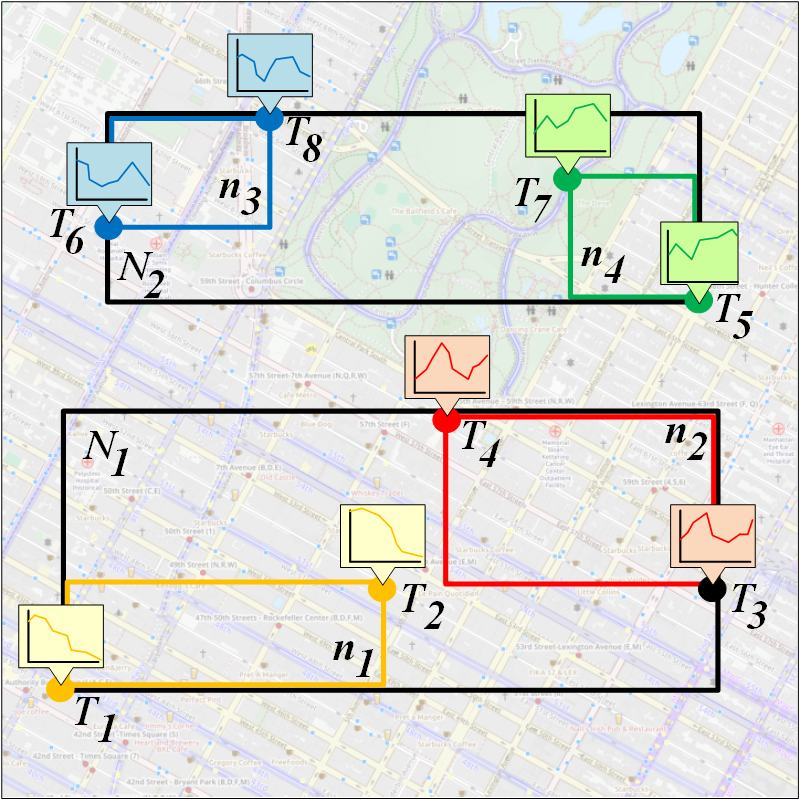
\includegraphics[width=42mm]{Figures/geotimeseries.png}\label{subfig:sample}}
 \end{minipage}
\begin{minipage}[!t]{0.4\linewidth}
\subfloat[Spatial-only R-tree index]{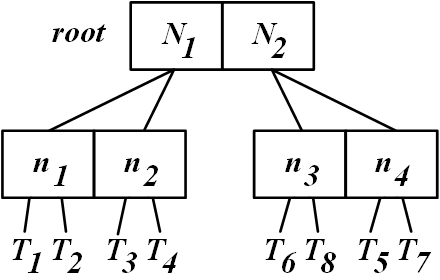
\includegraphics[width=34mm]{Figures/r_tree.png}\label{subfig:rtree}} \\
\subfloat[Hybrid \btsr index]{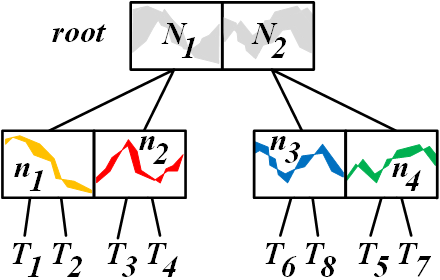
\includegraphics[width=34mm]{Figures/btsr_tree.png}\label{subfig:btsrtree}}
\end{minipage}
 \vspace{-10pt}
\caption{The \btsr index.}
\label{fig:example}
\end{figure}
% }

\subsubsection{Problem Definition}
\label{subsec:prob_def}

We first define the local similarity between time series, and then present the query variants we consider in this paper.

% \noindent \textbf{\emph{Time Series Local Similarity.}} Two time series are considered locally similar if they have similar values over some time intervals of significant duration. More specifically:

% \begin{mydefinition}[Locally Similar Time Series]
% Two time series $X$ and $X'$ are locally similar with respect to parameters $\delta$ and $\epsilon$, if there exists a time interval $I$ spanning at least $\delta$ consecutive timestamps, such that at every timestamp in $I$ their corresponding values do not differ by more than $\epsilon$, i.e., $\forall t \in I, |X^{t} - X'^{t}| \leq \epsilon$ and $|I| \geq \delta$.
% \end{mydefinition}

\begin{mydefinition}[Local Time Series Similarity]
The {\em local similarity score} $\sigma$ between two time series $T$ and $T'$ is the maximum count of consecutive timestamps during which the respective values of $T$ and $T'$ do not differ by more than a given margin $\epsilon$, i.e., $\sigma(T, T', \epsilon) = |I_{max}|$, where $I_{max}$ is the longest consecutive time interval $I$ such that $\forall i \in I, |T^{i} - T'^{i}| \leq \epsilon$.
\end{mydefinition}

%\noindent \textbf{\emph{Time Series Local Similarity Score.}} We define the local similarity score among a pair of co-evolving time series, that is the number of consecutive time stamps they are locally similar. More formally:

%\begin{mydefinition}[Local Similarity Score]
%Given two locally similar co-evolving time series $X$ and $X'$ and the set of the corresponding local similarity intervals $\mathcal{SI}$, their local similarity score is the total duration of all the intervals in $\mathcal{I}$:

%\begin{equation} \label{eq:local_score}
%d_{ls}(X, X') = \sum_{m=1}^{|\mathcal{SI}|} |I_m|.
%\end{equation}
%\end{mydefinition}

% \noindent \textbf{\emph{Problem Definition.}}
In this work, our goal is to efficiently support hybrid queries on geolocated time series that retrieve the results based both on spatial proximity and local similarity. Specifically, we focus on the following types of queries (hereafter referred to as \textit{LS-queries}):

\begin{itemize}
    \item $Q_{rr}(T_q, \rho, \epsilon, \delta)$: Given a geolocated time series $T_q$, retrieve every geolocated time series $T$ such that $T$ is located within range $\rho$ from $T_q$, i.e., $d(T_q, T) \leq \rho$ and has local similarity to $T_q$ at least $\delta$, i.e., $\sigma(T_q, T) \geq \delta$.
    \item $Q_{kr}(T_q, k, \epsilon, \delta)$: Given a geolocated time series $T_q$, retrieve the spatial $k$-nearest neighbors to $T_q$ that also have local similarity to $T_q$ at least $\delta$.
    \item $Q_{rk}(T_q, \rho, \epsilon, k)$: Given a geolocated time series $T_q$, retrieve the top-$k$ geolocated time series that have the highest local similarity to $T_q$ with respect to $\epsilon$ and are located within range $\rho$ from $T_q$.
\end{itemize}

\begin{myexample}
 Figure \ref{fig:example_query} depicts an example of the $Q_{rr}(T_q, \rho, \epsilon, \delta)$ query. Given the geolocated time series $T_q$ as query, we seek the spatially close ones (i.e., within a circle of radius $\rho$) that are also locally similar within margin $\epsilon$ for at least $\delta$ timestamps. In this example, despite five geolocated time series being within range, only $T_2$ and $T_7$ qualify for the final result, since these are the ones that are also locally similar for at least one time interval of length at least $\delta$.
\end{myexample}

\begin{comment}
\begin{figure}[!t]
 \centering
 \subfigure[Geolocated time series within $\epsilon_{sp}...$]{\includegraphics[width=50mm]{Figures/spatial_prox.png}\label{subfig:spatial_proximity}}
 \subfigure[...that are also locally similar.]{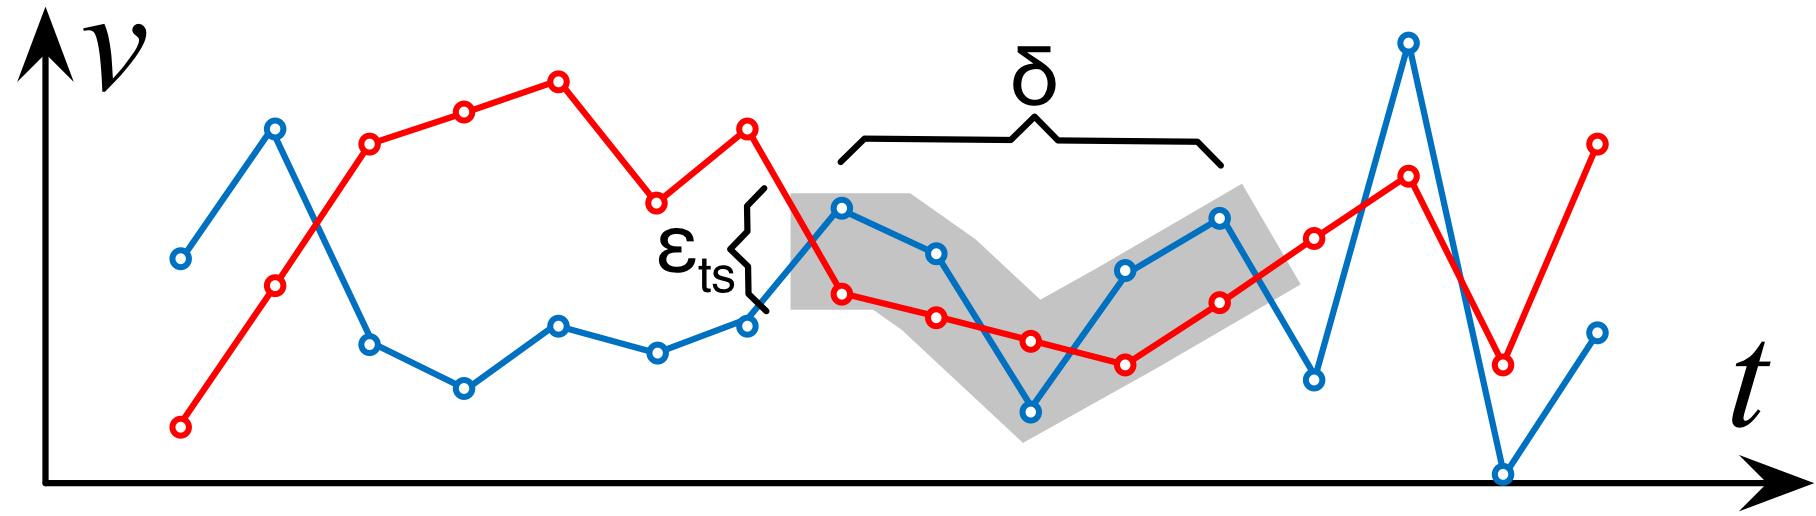
\includegraphics[width=75mm]{Figures/local_sim.png}\label{subfig:local_sim}}
 \vspace{-10pt}
\caption{$Q^{LS}_{r}$ query on geolocated time series.}
\label{fig:example_query}
\end{figure}
\end{comment}